\documentclass[11pt]{article}

\usepackage{amsmath,amsfonts,amssymb}
\usepackage{breqn}
\usepackage[pdftex]{graphicx}
\usepackage{natbib}
\usepackage[usenames,dvipsnames]{xcolor}
%\usepackage[nooneline,tight,raggedright]{subfigure}
\usepackage{multirow}
\usepackage[version=3]{mhchem}

\usepackage{wrapfig}
\usepackage{pstricks,enumerate}
\usepackage{colortbl}
\usepackage{hhtensor}
\usepackage{longtable}
\usepackage[hang,flushmargin,symbol*]{footmisc}
\usepackage[]{algorithm2e}

\usepackage[font=footnotesize,format=plain,labelfont=bf]{caption}
\usepackage{subcaption}

%%%%%%%%% PAGE DIMENSIONS


\setlength{\oddsidemargin}{-0.5in}
\setlength{\textwidth}{5.0in}
\setlength{\topmargin}{-0.5in}
\setlength{\footskip}{0.30in}
\setlength{\textheight}{9.0in}
\setlength{\headheight}{0.2in}
\setlength{\headsep}{0.3in}

%%%%%%%%% SECTIONING STUFF
\makeatletter
\renewcommand{\section}{\@startsection
{section}%
{0}%
{0mm}%
{0.4\baselineskip}%
{0.4\baselineskip}%
{\normalfont\Large\bfseries\color{myBrown}}}%
\makeatother

\makeatletter
\renewcommand{\subsection}{\@startsection
{subsection}%
{1}%
{0mm}%
{0.4\baselineskip}%
{0.4\baselineskip}%
{\normalfont\large\bfseries\color{myBrown}}}%
\makeatother

\makeatletter
\renewcommand{\subsubsection}{\@startsection
{subsubsection}%
{1}%
{0mm}%
{-0.5\baselineskip}%
{0.3\baselineskip}%
{\normalfont\normalsize\itshape\centering\color{myBrown}}}%
\makeatother




\renewcommand{\thesection}{\arabic{section}}
\renewcommand{\thesubsection}{\thesection.\arabic{subsection}}

%\renewcommand*{\thefootnote}{\fnsymbol{footnote}}
%\renewcommand{\footnoterule}{%
%  \kern -3pt
% \hrule width \textwidth height 1pt
%  \kern 2pt
%}

%%%%%%%%% FORMATTING TIDBITS

\definecolor{myTan}{RGB}{205,133,63}
\definecolor{myBrown}{RGB}{155,77,40}
\captionsetup{labelfont={color=myBrown,bf},textfont={color=myTan}}
\newcommand{\HRule}[2]{{\color{myBrown}\rule{#1}{#2}}}
\newcommand{\tPI}[1]{{\color{myBrown}#1}}
\newcommand{\sPI}[1]{\textsc{\color{myBrown}#1}}
\newcommand{\cPI}[1]{\textbf{\color{myBrown}#1}}
\newcommand{\iPI}[1]{\textit{\color{myBrown}#1}}
\newcommand{\lead}[1]{\textit{\color{myBrown}(#1)}}
\newcommand{\tabtit}[1]{\textsc{\color{myBrown}#1}}
\newcommand{\entry}[1]{\mbox{\sffamily\bfseries{#1:}}\hfil}%
\newcommand{\bitem}{\item[{\color{myBrown}$\bullet$}]}
\newcommand{\bmath}{\boldsymbol}
\newcommand{\eps}{\varepsilon}
\newcommand{\Dpartial}[2]{\frac{\partial #1}{\partial #2}}
\newcommand{\itemcolor}[1]{% Update list item colour
\renewcommand{\makelabel}[1]{\color{#1}\hfil ##1}}
\newcommand{\PlasComCM}{\textit{PlasComCM}}
\newcommand{\cl}[1]{\textit{codelet-#1}}
\newcommand{\Cl}[1]{\textit{Codelet-#1}}
\newcommand{\fut}{$^*$}
\newcommand{\pas}{$^\dag$}
\newcommand{\plusplus}[1]{#1{}\texttt{++}}
%%
%%
\newif\ifclean
\cleantrue
%\cleanfalse

%%%%% CONSISTENCY COMMANDS
\newcommand{\eqr}[1]{(\ref{#1})}
\newcommand{\fgr}[1]{figure~\ref{#1}}
\newcommand{\tbr}[1]{Table~\ref{#1}}
\newcommand{\Fgr}[1]{Figure~\ref{#1}}
\newcommand{\secr}[1]{section~\ref{#1}}
\newcommand{\eqnd}[2]{equations~(\ref{#1}) and (\ref{#2})}
\newcommand{\pp}[1]{\ensuremath{\left( #1 \right)}}
\newcommand{\psq}[1]{\ensuremath{{\left[ #1 \right]}}}
\newcommand{\pcrl}[1]{\ensuremath{{\left \{ #1 \right \} }}}
\newcommand{\pang}[1]{\ensuremath{ \left \langle #1 \right \rangle }}
\providecommand{\pop} {}
\renewcommand{\pop}[2] {\ensuremath{\frac {\partial{#1}} {\partial{#2}}} }
\newcommand{\popn}[3] {\ensuremath{\frac {\partial^{#3}{#1}} {\partial{#2}^{#3}}} }
\newcommand{\dod}[2] {\ensuremath{\frac {d{#1}} {d{#2}}} }
\newcommand{\nd}{\ensuremath{~\textrm{and}~}}
\newcommand{\ee}[1]{ \ensuremath{\times 10^{#1}}} 
\newcommand{\plasma}{\ensuremath{\mathrm{c}}}
\newcommand{\plasmar}{\ensuremath{\mathrm{cr}}}
\newcommand{\dancode}{\emph{PlasComCM}}
\newcommand{\bvec}[1]{\ensuremath{\boldsymbol{#1}}}
\newcommand{\mat}[1]{\ensuremath{\mathsf{#1}}}
\newcommand{\parab}[2]{\vspace{#1 pt}\noindent \paragraph{\bf #2 \\}}
\newcommand{\answer}[1]{
$$
\begin{array}{|c|}\hline \\
#1 \\
\\ \hline
  \end{array}
$$}
\newcommand{\Answer}[1]{
\ensuremath{
\begin{array}{|c|}\hline \\
#1 \\
\\ \hline
  \end{array}}}

\DeclareMathOperator\erf{erf}

\usepackage[toc,page]{appendix}
\usepackage{fancyvrb}
% redefine \VerbatimInput
\RecustomVerbatimCommand{\VerbatimInput}{VerbatimInput}%
{fontsize=\tiny,
 %
 frame=lines,  % top and bottom rule only
 framesep=2em, % separation between frame and text
 rulecolor=\color{Gray},
 %
}


%%%%%%%%% COMMENTS/INSTRUCTIONS/NOTES
\setlength{\marginparwidth}{.65in}
\newcommand{\margcomment}[1]{{\color{red}$\bullet$}\marginpar{\raggedright
{\color{red} \tiny #1}}}
\newcommand{\TODO}[1]{{\color{blue}$\bullet$}\marginpar{\raggedright
{\color{blue} \tiny TODO: #1}}}
\usepackage[disable,colorinlistoftodos, color=blue!20!white, bordercolor=gray,
textsize=tiny,textwidth=2.7in]{todonotes}
\newcommand{\LOGM}[1]{\todo[noline,color=green!40]{Luca: #1}}
\newcommand{\LOGF}[1]{\todo[noline,color=orange!40]{JBF: #1}}
\usepackage{color,soul}
\newcommand{\hly}[1]{\textcolor{blue}{#1}}
\usepackage{pstool}
%%%%%%%%%%%%%%%%%%%%%%%%%




%%%%%%%%NOMENCLATURE



%%%% REMOVE COMMENTS
\renewcommand{\hl}{}
\renewcommand{\hly}{}
\setlength{\oddsidemargin}{00.0in}
\setlength{\textwidth}{6.5in}

\begin{document}
\pagestyle{plain}

Hi Dan, and Lukas,

After today's discussions, I am convinced we should be able to integrate Lukas' \textit{OpenCL}-based strategy for accelerator/cpu integration with the PC2 development codelets with minimal effort. This is low-hanging fruit and I believe we should jump on it. If you agree, I'd like to discuss some of the specific details about how each of our codes work and make a plan for integration upon which we can all agree. I am just hoping to start a discussion here, not provide a complete description.

Figures~\ref{Figure:Lukas1}, \ref{Figure:Lukas2} and \ref{Figure:PC2Codelet1} are cartoons of my understanding of the \textit{OpenCL} code (does it have a proper name?) and \textit{PlasCom2} development codelets. Lukas, please comment and/or correct this if it's off-base. My understanding of the \textit{OpenCL} procedure is as follows:

\begin{enumerate}
\item{Initialization} -- the domain is coarsely partitioned, the CPU and GPU regions are ``decided'', MPI processes \textbf{P} and \textbf{M} are created to \textit{handle} the CPU and GPU regions, respectively. Process \textbf{P} runs a regular \plusplus{C} program, while the GPU handler process \textbf{M} runs an \textit{OpenCL} program. The GPU/CPU and CPU/CPU halo regions are formed, and all partition buffers are created to \textbf{include} the halo regions. All initial data is exchanged so that the overall program is ready to begin stepping.
\item{Step}\label{step:step} --  Each process \textbf{P} conducts the $N$th RBSOR step, using the already available remote halo data in its main buffer. OpenMP loop parallelism is used to thread the procedure and distribute to available processing cores on the host platform. At the same time, GPU handler processes \textbf{M} use blocking \textit{OpenCL} directives to advance the solution owned by the accelerator devices.
\item{Communication collection \& send} -- Each CPU process \textbf{P} copies the local halo data (i.e. that required by remote (CPU and GPU) partitions) into MPI send buffers, and sends (non-blocking) to remote processes (including remote processes of type \textbf{P} and \textbf{M}. Each GPU process copies local halo data into local buffers dedicated to communication with its driver process \textbf{M}. The GPU driver process \textbf{M} pulls the halo data from the GPU using \textit{OpenCL} directives, and packs the data into MPI communication buffers which it uses to send to remote processes (including the local parent of type \textbf{P}, and remote processes of types \textbf{P} and \textbf{M}.
\item{Receive and unpack} -- All MPI processes of all types post matching receives to all the posted sends, and perform unpacking of the received data into local main buffers. For processes of type \textbf{M}, the data is pushed to the device exchange buffer, and then from the device exchange buffer into the device partition's main buffer using blocking \textit{OpenCL} directives.
\item{Update N} - Go to Step~\ref{step:step}
\end{enumerate}

I propose that we do a few of things: 
\begin{description} 
\item{Update Lukas' OpenCL code} -- Port the advection kernels from the PC2 development codelets and RK4 to the OpenCL integrator, and conduct the verification test on the results. Currently, we only really know that the OpenCL integrator doesn't fail to run.  We have a one-file, flat procedural implementation of the 1dadvection that should be quite easy to port to Lukas' framework. This will also give us an idea of what it takes to implement the time-marching driver in the \textit{OpenCL} program run by MPI processes of type \textbf{M}.
\item{Update Codelet 4 to use OpenCL} -- The general plan would be to take the interior part of the partition interval, $\text{\mathbf{I}}$, and dispatch it to the GPU through using Lukas' mechanism of spawning off an MPI process of type \textbf{M} to manage the GPU through \textit{OpenCL}. The CPU part of the partition interval would likely retain only the local halo regions, $\text{\mathbf{B}}_{i}$, and domain boundaries. The fact that some remote processes are of type \textbf{M} and handle GPU devices should be transparent to the current operation of Codelet 4. 
\end{description}

There are a few additional things we should discuss about using asynchronous communication and asynchronous \textit{OpenCL} to overlap communciation and computation for further gains in Lukas' code, as well as to jibe with the current Codelet4 control flow. Lukas and I have reviewed a potential control flow, and identified a couple of minor related buffering issues.  More details on this can be provided as our discussions continue (if we agree they should continue).

\begin{figure}[h]
\begin{center}
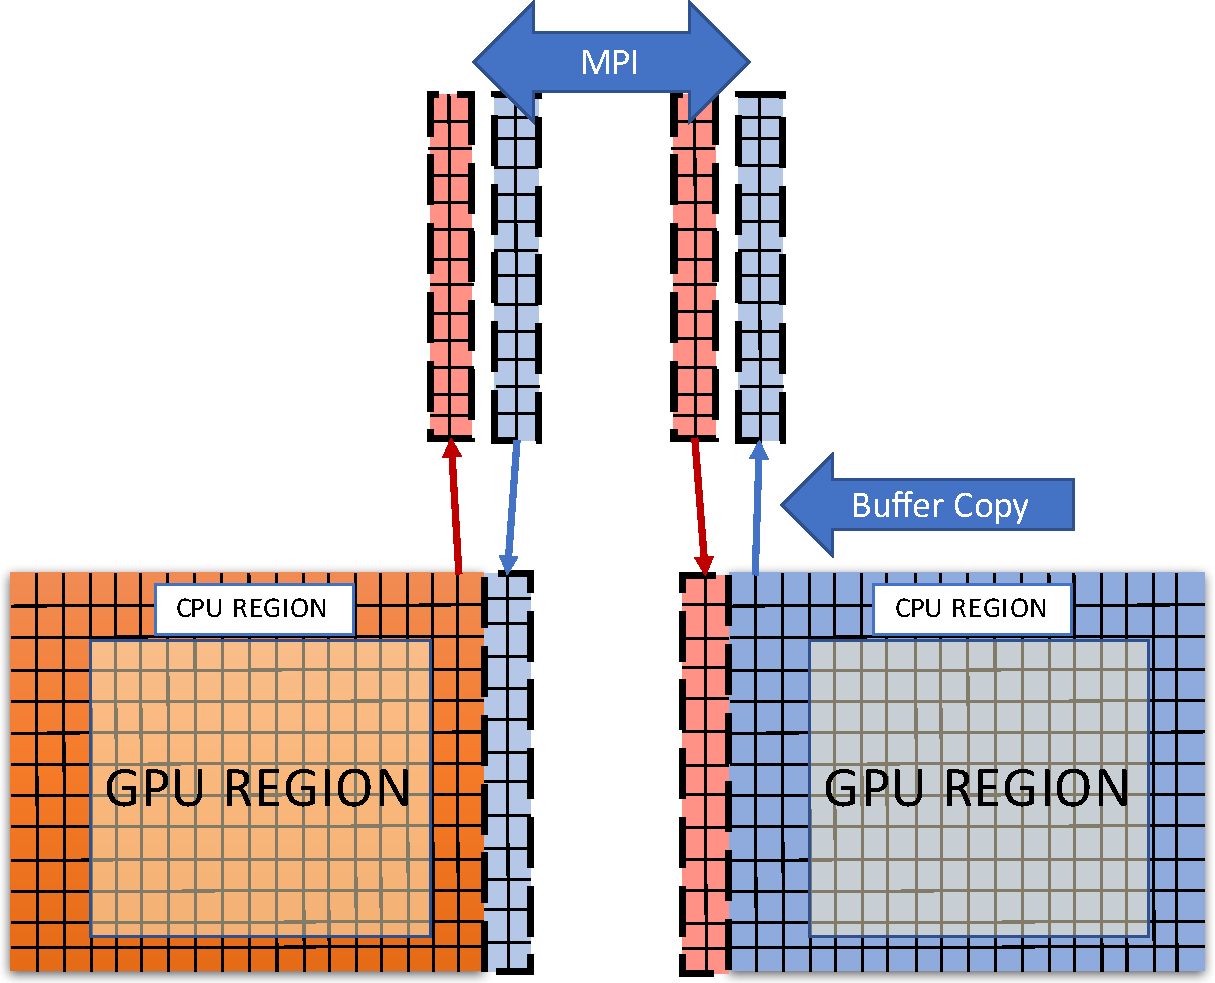
\includegraphics[width=\textwidth]{Figures/Lukas1}
\vspace{-20pt}
\caption{Partition arrangements and communication buffers for OpenCL integrator. An initial \textit{coarse} partitioning into some number of partitions is followed by a finer partitioning of each coarse partition where some subset of the partition is sent to a GPU. In general, the GPU region may collide with the coarse partition boundary, but in practice it may be better if it does not. Each MPI process that handles some portion of the domain (i.e. some partition), communicates data in the halo regions by performing copies to-and-from communication buffers that are used in MPI exchanges. The grid and state buffers are allocated such that they \textit{include} the remote halo regions (i.e. the regions that will contain data owned by remote partitions).}\label{Figure:Lukas1}
\end{center}
\end{figure}


\begin{figure}[h]
\begin{center}
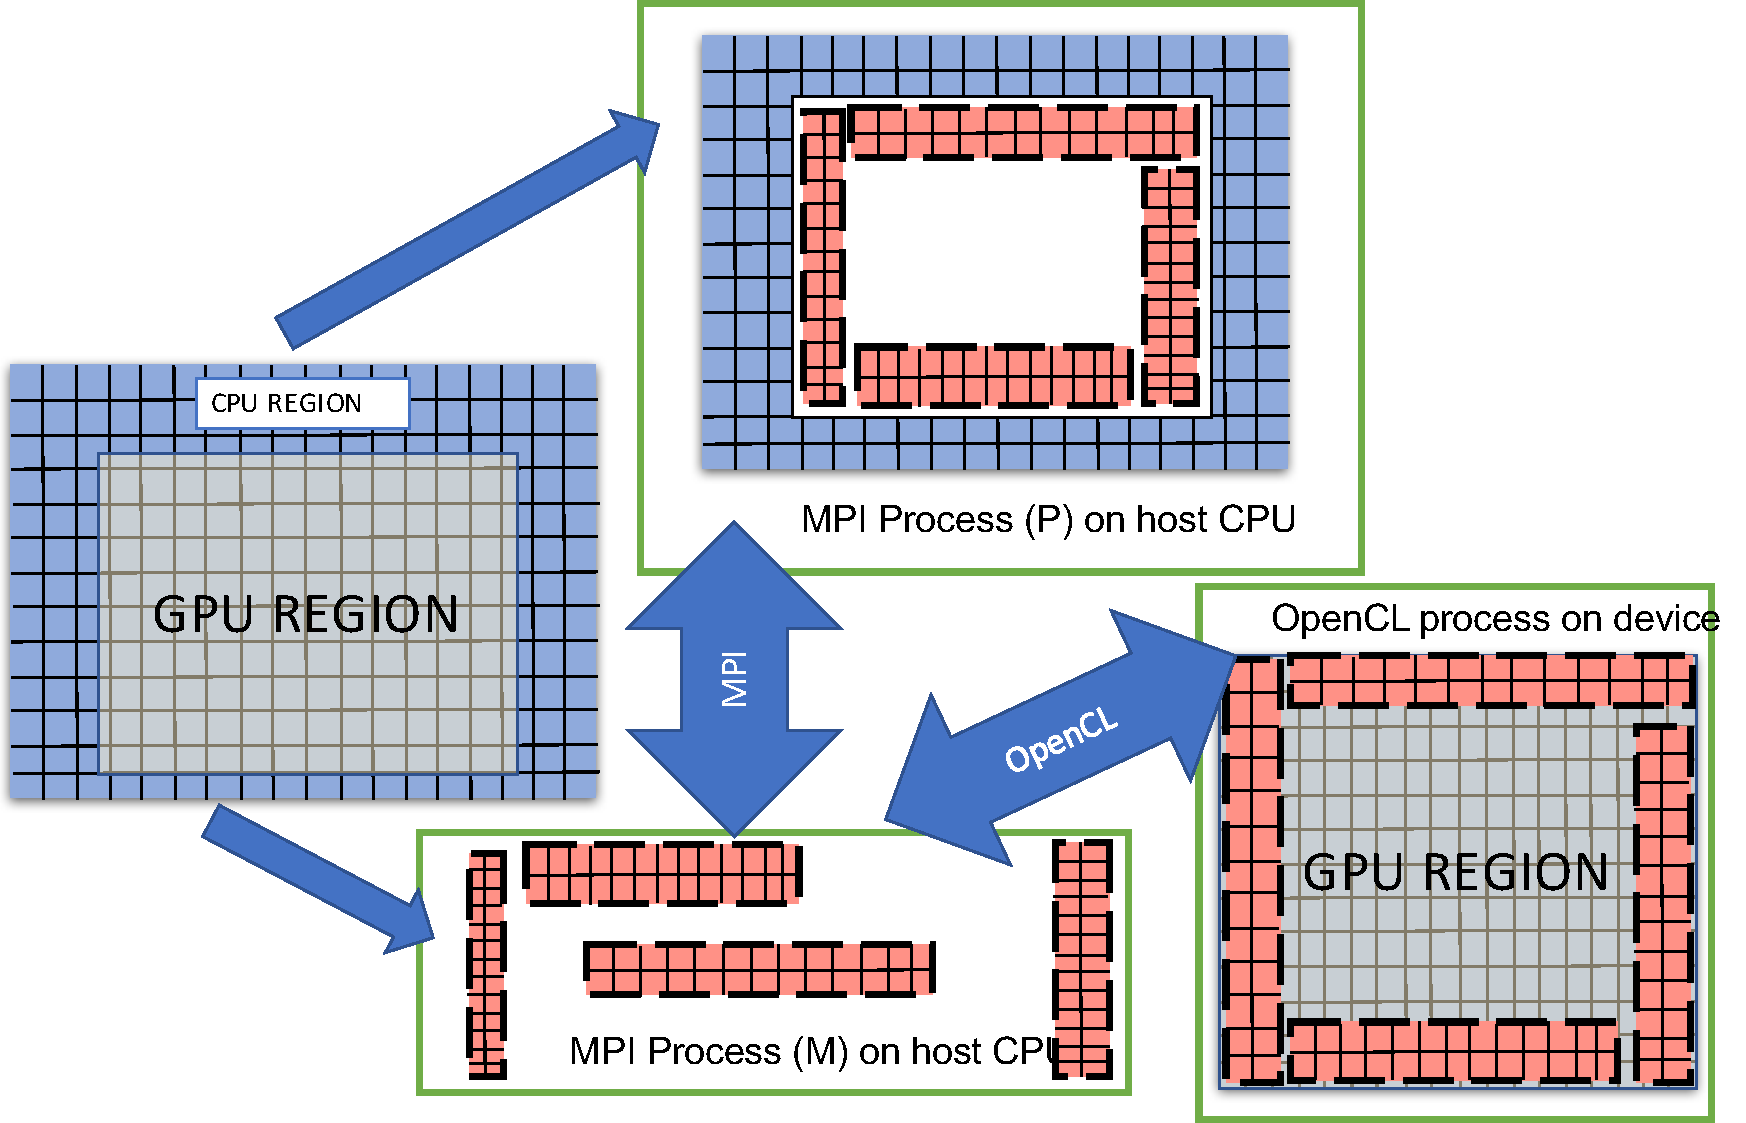
\includegraphics[width=\textwidth]{Figures/Lukas2}
\vspace{-20pt}
\caption{Details of single coarse partition of the OpenCL integrator -- \textit{work} partitioning. The CPU region(s) (possibly a disparate collection of them) are handled by MPI process \textbf{P} on the compute host, and the GPU region (a contiguous subset of the coarse partition) is handled by MPI process \textbf{M} on the compute host. MPI process \textbf{M} is simply a \textit{handler} for \textit{OpenCL} program that runs on the device. The handler process owns the MPI communication buffers used in communicating the gpu/cpu halos between the two host-local MPI processes, and manages the control flow of the \textit{OpenCL} program.  If the GPU region actually collides with the coarse partition boundaries, then the handler process is capable of sending data directly to the corresponding MPI process that requires the halo data. GPU/CPU communication and control flow handling between the \textit{OpenCL} program and the MPI process \textbf{M} are acutated by \textit{OpenCL} directives, and involves the same copy,transfer,copy sequence used in the MPI-MPI exchanges.}\label{Figure:Lukas2}
\end{center}
\end{figure}

\begin{figure}[h]
\begin{center}
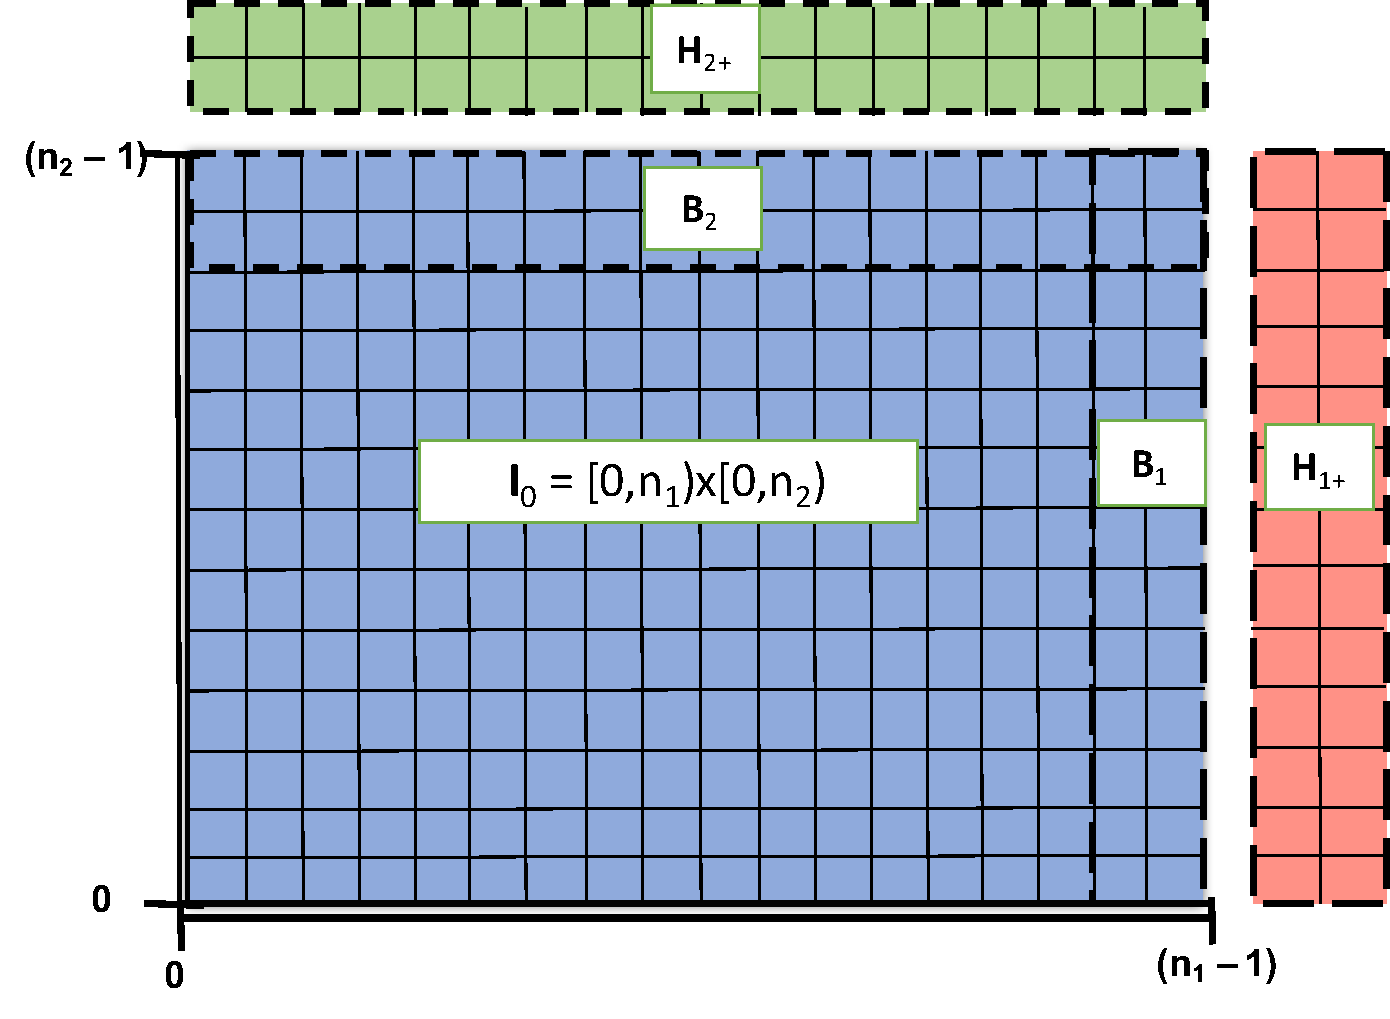
\includegraphics[width=\textwidth]{Figures/PC2Codelet1}
\vspace{-20pt}
\caption{PlasCom2 development codelet partition arrangements, regions, and communication regions. In Codelets 3 \& 4, multiple levels of partitioning result in a set of partition intervals, ${\text{\mathbf{I}}_p}$. The grid and state buffers are allocated such that the \textit{remote halo regions} specified by intervals $\text{\mathbf{H}}_{i^{\pm}}$ are not included. The \textit{local halo regions} specified by intervals $\text{\mathbf{B}}_{i^{\pm}}$ are the regions in the local partition that are required by remote partitions. For each region that requires communication with remote partitions, matching send and receive buffers are created.}\label{Figure:PC2Codelet1}
\end{center}
\end{figure}



\end{document}
%-------------------------------------------------------------------------
